
\section{Inverse Problems}
\label{sec:inverse-problems}

The problem of determining PDFs from a set of experimental data falls under the
general category of {\em inverse problems}, \ie\ the problem of finding the
input to a given model knowing a set of observations, which are often finite and
noisy. In this section we are going to review the Bayesian formulation of
inverse problems. It is impossible to do justice to this vast subject here.
Instead we try to emphasise the aspects that are relevant for quantifying
uncertainties on PDF determinations. 

\subsection{Statement of the problem}
\label{sec:BayesianInverse}

The space of inputs is denoted by $\modelspace$, while $R$ denotes the space of
responses. The model is specified by a {\em forward map}
\begin{align}
  \label{eq:ForwardMap}
  \fwdmapop : ~& \modelspace \to R \nonumber \\
      & \modelvec \mapsto r=\fwdmapop(\modelvec) \, ,
\end{align}
which associates a response $r \in R$ to the input $\modelvec \in \modelspace$,
where we assume that $\modelspace$ and $R$ are Banach spaces.~\footnote{Banach
spaces are complete normed vector spaces. We do not need to get into a more
detailed discussion here, but it is important to note that working in Banach
spaces allows us to generalise the results to infinite-dimensional spaces of
functions.} As an example we can think of $\modelvec$ as being a PDF, \ie\ a
function defined on the interval $[0,1]$, and $r$ a DIS structure function. The
structure function is related to the PDF by a factorization formula involving
perturbative coefficient functions: 
\begin{align}
  \label{eq:DISExample}
  r(x,Q^2) = \int_x^1 \frac{dz}{z}\, C(z,Q^2) \modelvec(x/z,Q^2)\, .
\end{align}
Note that in this example the forward map maps one real function into another
real function. In this case the space of models $X$ is the space of continuous
functions defined on the interval $[0,1]$, which satisfy integrability
conditions. Even though this is an infinite-dimensional space, it is possible to
define a probability measure on such a space and construct a Bayesian solution
to the inverse problem. In current determinations of PDFs, the functional form
of the PDF is dictated by some kind of parametrization, with different
parametrizations being used by different collaborations. In all cases, the space
$X$ is a finite-dimensional space, $\real^{\nmodel}$, where $\nmodel$ is
the number of parameters. In the case of the NNPDF fits discussed below, the
weights of the neural networks are the parameters that determine the functional
form of the PDFs. Alternatively, one could think of a finite-dimensional
representation defined by the value of the PDF at selected values of $x$, \ie\
$u_i=u(x_i)$ for $i=1,\ldots,\nmodel$. Depending on the context we will denote
by $u$ either the function $u(x)$, or the vector of real parameters that are
used to determine the function $u(x)$. Disambiguation should hopefully be
straightforward. 

Experiments will not have access to the full function $r$ but only to a subset
of $\ndata$ observations. In order to have a formal mathematical expression that
takes into account the fact that we have a finite number of measurements, we
introduce an {\em observation operator}
\begin{align}
  O : ~& R \to Y \nonumber \\
       & r \mapsto \obs \, ,
\end{align}
where $\obs \in Y$ is a vector in a finite-dimensional space $Y$ of experimental
results, \eg\ the value of the structure function for some values of the
kinematic variables $x$ and $Q^2$. In general we will assume that $\obs \in
\real^{\ndata}$, \ie\ we have a finite number $\ndata$ of real experimental
values. The quantity of interest is the composed operator
\begin{align}
  \fwdobsop : ~& \modelspace \to \real^{\ndata} \nonumber \\
                 & \fwdobsop = O \circ G\, ,
\end{align}
which maps the input $\modelvec$ to the set of data. Taking into account the
fact that experimental data are subject to noise, we can write
\begin{align}
  \label{eq:NoisyInverseProblem}
  \obs = \fwdobsop(\modelvec) + \obsnoise\, ,
\end{align}
where $\obsnoise$ is a random variable defined over $\real^{\ndata}$ with
probability density $\rho(\obsnoise)$. We will refer to $\obsnoise$ as the {\em
observational noise}. In this setting, the inverse problem becomes finding
$\modelvec$ given $\obs$. It is often the case that inverse problems are
ill-defined in the sense that the solution may not exist, may not be unique, or
may be unstable under small variations of the problem. 

In solving the inverse problem, we are going to adopt a Bayesian point of view,
as summarised \eg\ in Ref.~\cite{Stuart:2010}: our prior knowledge about
$\modelvec$ is encoded in a prior probability measure $\mu_X^0$, where the
suffix $X$ indicates that the measure is defined in the space of models, and the
suffix 0 refers to the fact that this is a prior distribution. We use Bayes'
theorem to compute the posterior probability measure of $\modelvec$ given the
data $\obs$, which we denote as $\mu_X^\fwdobsop$. When the probability measure
can be described by a probability density, we denote the probability densities
associated to $\mu_X^0$ and $\mu_X^\fwdobsop$, by $\pi_X^0$ and
$\pi_X^\fwdobsop$ respectively. Then, using Eq.~(\ref{eq:NoisyInverseProblem}),
we can write the data likelihood, \ie\ the probability density of $\obs$ given
$\modelvec$,
\begin{align}
  \label{eq:YGivenUProbDensity}
  \pi_Y(\obs|\modelvec) = \rho(\obs-\fwdobsop(\modelvec))\, ,
\end{align}
and Bayes' theorem yields
\begin{align}
  \label{eq:BayesThmInversePosterior}
  \pi_X^\fwdobsop(\modelvec) = \pi_X(\modelvec|\obs) \propto 
  \pi_X^0(\modelvec)
  \rho(\obs-\fwdobsop(\modelvec))\, .
\end{align}

Even though the concepts that we have introduced so far should sound familiar,
it is worthwhile clarifying some ideas and present an explicit case where all
the probability densities are carefully defined. This is best exemplified by
considering the case where both the observational noise and the model prior are
Gaussian. We assume that we are given a set of central values $\obspriorcent \in
\real^{\ndata}$ and their covariance matrix $\obspriorcov$. Then the {\em prior}
probability density of the observable $\obs$ is 
\begin{equation}
  \label{eq:PriorData}
  \pi_{Y}^0(\obs|\obspriorcent,\obspriorcov) \propto \exp\left(
    -\frac12 \left| \obs - \obspriorcent \right|_{\obspriorcov}^2
    \right)\, ,
\end{equation}
where, similarly to the convention used above, the suffix $Y$ emphasises the
fact that this is a probability density in data space, and the notation
explicitly reminds us that this is the probability density given the central
values $\obspriorcent$ (and the covariance matrix $\obspriorcov$). Similarly we
can choose a Gaussian distribution for the prior distribution of the input
model, characterized by a central value $\modelpriorcent$ and a covariance
$\modelpriorcov$:
\begin{align}
  \label{eq:PiZeroGauss}
  \pi_{X}^0(\modelvec|\modelpriorcent,\modelpriorcov)  
  &\propto \exp\left(
              -\frac12 \left| \modelvec - \modelpriorcent \right|_{\modelpriorcov}^2
              \right)\, .
\end{align}
Following the convention above, we use a suffix $X$ here to remind the reader
that we are looking at a probability density in the space of models. Note that
in the expressions above we used the norms in $\modelspace$ and $\real^{\ndata}$
respectively, and introduced the short-hand notation
\begin{align}
  \left|a\right|_M^2 = \left| M^{-1/2} a\right|^2\, ,
\end{align}
where $a$ denotes a generic element of $\modelspace$, $R$ or $\real^{\ndata}$.
For the case where $a \in \real^{\ndata}$, we use the Euclidean norm and
\begin{align}
  \left| a \right|_M^2 = \sum_{i,j} a_i M^{-1}_{ij} a_j\, ,
\end{align}
where the indices $i,j$ run from 1 to $\ndata$, which eventually yields the
usual expression for the $\chi^2$ of correlated data.   
Up to this point data and models are completely independent, and the joint
distribution is simply the product of $\pi_{Y}^0$ and $\pi_{X}^0$. 

The forward map induces a correlation between the input model and the
observables, so we introduce a probability density $\theta$ that describes these
correlations due to the underlying theory,  
\begin{equation}
  \label{eq:ThetaCorr}
  \theta(\obs,\modelvec|\fwdobsop) = \delta\left(\obs - \fwdobsop(\modelvec)\right)\, ,
\end{equation}
where the Dirac delta corresponds to the case where there are no theoretical
uncertainities. Theoretical uncertainties can be introduced by broadening the
distribution of $\obs$ away from the exact prediction of the forward map, \eg\
using a Gaussian with covariance $C_T$,
\begin{equation}
  \label{eq:TheoryErrors}
  \theta(\obs,\modelvec|\fwdobsop) = \exp\left(
    -\frac12 
    \left| \obs - \fwdobsop(\modelvec)
    \right|_{C_T}^2\right)\, .
\end{equation}
In the context of PDF fitting a similar recipe to take into account theoretical
errors has recently been advocated in
Refs.~\cite{NNPDF:2019vjt,AbdulKhalek:2019ihb}. Note that there are no rigorous
arguments favouring the assumption that theoretical errors are normally
distributed; it is nonetheless a useful working assumption, and a definite
improvement compared to ignoring the theoretical errors altogether. The net
effect of the theory errors is a redefinition of the covariance of the data,
which has no major impact in our discussion, and therefore will be ignored.
Taking the correlation $\theta(\obs,\modelvec|\fwdobsop)$ into account, the
joint distribution of $\obs$ and $\modelvec$ is
\begin{align}
  \label{eq:JointYAndU}
  \pi^\fwdobsop(\obs,\modelvec|\obspriorcent,\obspriorcov,\modelpriorcent,\modelpriorcov) 
  \propto 
  \pi_{X}^0(\modelvec|\modelpriorcent, \modelpriorcov) 
  \pi_{Y}^0(\obs|\obspriorcent,\obspriorcov) 
  \theta(\obs,\modelvec|\fwdobsop)\, .
\end{align}
We can now marginalize with respect to \obs, neglecting theory errors, 
\begin{align}
  \label{eq:MarginOne}
  \pi^\fwdobsop_{X}(\modelvec|\obspriorcent,\obspriorcov,\modelpriorcent,\modelpriorcov) 
  &\propto \int dy\, 
    \pi_{X}^0(\modelvec|\modelpriorcent,\modelpriorcov) 
    \pi_{Y}^0(\obs|\obspriorcent,\obspriorcov) 
    \theta(\obs,\modelvec|\fwdobsop) \\
  & \propto \pi_{X}^0(\modelvec|\modelpriorcent,\modelpriorcov)  
    \int dy\, 
    \pi_{Y}^0(\obs|\obspriorcent,\obspriorcov) 
    \delta\left(\obs-\fwdobsop(\modelvec)\right) \\
  & \propto 
    \pi_{X}^0(\modelvec|\modelpriorcent,\modelpriorcov) \,
    \pi_{Y}^0(\fwdobsop(\modelvec)|\obspriorcent,\obspriorcov)\, .
\end{align}
We see that we have recovered Eq.~\ref{eq:BayesThmInversePosterior}. The
log-likelihood in the Gaussian case is simply the $\chi^2$ of the data,
$\obspriorcent$, to the theory prediction, $\fwdobsop(\modelvec)$:
\begin{equation}
  \label{eq:LikelyChiSq}
  -\log\pi_{Y}^0(\fwdobsop(\modelvec)|\obspriorcent,\obspriorcov) =  
    \frac12 \sum_{i,j=1}^{\ndata}
      \left(\fwdobsop(\modelvec) - \obspriorcent \right)_i
      \left(\obspriorcov^{-1}\right)_{ij}
      \left(\fwdobsop(\modelvec) - \obspriorcent \right)_j
    \, .
\end{equation}
In the notation of Eq.~\ref{eq:BayesThmInversePosterior}
\begin{equation}
  \label{eq:IdentifyRho}
  \pi_{Y}^0(\fwdobsop(\modelvec)|\obspriorcent,\obspriorcov) = \rho\left(
    \fwdobsop(\modelvec) - \obspriorcent
  \right)\, ,
\end{equation}
where in this case 
\begin{align}
  \label{eq:RhoGauss}
  \rho(\obsnoise) &\propto \exp\left(
               -\frac12 \left|\obsnoise\right|_{\obspriorcov}^2
               \right)\, .
\end{align}
The probability density $\pi^\fwdobsop_{X}(\modelvec|\obspriorcent,
\obspriorcov,\modelpriorcent,\modelpriorcov)$ was called
$\pi_{X}^\fwdobsop(\modelvec)$ in Eq.~\ref{eq:BayesThmInversePosterior}, where
the suffix $\fwdobsop$ is a short-hand to denote the posterior probability in
model space, taking into account all the conditional variables. Hence, for the
Gaussian case, the result from Bayes' theorem reduces to
\begin{align}
  \label{eq:PosteriorModel}
  \pi_{X}^\fwdobsop(\modelvec) 
  &\propto 
  \exp\left[
    -\frac12 \left| \obspriorcent - \fwdobsop(\modelvec) \right|_{\obspriorcov} ^2
    -\frac12 \left| \modelvec - \modelpriorcent \right|_{\modelpriorcov}^2
  \right] \\ 
  &\propto
  \exp\left[
    - S(\modelvec)
  \right]\, .
\end{align}
Note that in the argument of the likelihood function we have the central values
of the data points $\obspriorcent$ as given by the experiments.
Eq.~(\ref{eq:PosteriorModel}) is the Bayesian answer to the inverse problem, our
knowledge of the model $\modelvec$ is encoded in the probability measure
$\mu_{X}^\fwdobsop$, which is fully specified by the density
$\pi_{X}^\fwdobsop$. There are several ways to characterise a probability
distribution, a task that becomes increasingly difficult in high-dimensional
spaces. As discussed later in this study, the NNPDF approach is focused on the
determination of the {\em Maximum A Posteriori (MAP)} estimator, \ie\ the
element $u_* \in \modelspace$ that maximises $\pi_{X}^\fwdobsop(\modelvec)$:
\begin{align}
  \label{eq:MAP}
  u_* = \arg\min_{\modelvec \in \modelspace} 
  \left(
    \frac12 \left| \obspriorcent - \fwdobsop(\modelvec) \right|_{\obspriorcov}^2
    + \frac12 \left| \modelvec - \modelpriorcent \right|_{\modelpriorcov}^2
  \right)\, .
\end{align}
For every instance of the data $\obspriorcent$, the MAP estimator is computed by
minimising a regulated $\chi^2$, where the regularization is determined by the
prior that is assumed on the model $u$. We will refer to this procedure as the
{\em classical fit} of experimental data to a model. Note that in the Bayesian
approach, the regulator appears naturally after having specified carefully all
the assumptions that enter in the prior. In this specific example the regulator
arises from the Gaussian prior for the model input $\modelvec$, which is
normally distributed around a solution $\modelpriorcent$. The MAP estimator
provides the explicit connection between the Bayesian approach and the classical
fit.

\subsection{Comparison with classical fitting}
\label{sec:comp-class-fit}

Analytical results make the connection between the two approaches more
quantitative, and therefore more transparent. We are going to summarise these
results here without proofs, referring the reader to the mathematical literature
for the missing details. Working in the finite-dimensional case, we assume 
\begin{align*}
  \modelvec &\in \real^{\nmodel} \, ,\\
  \obs &\in \real^{\ndata}\, ,
\end{align*}
and we are going to review in detail two examples from Ref.~\cite{Stuart:2010},
which illustrate the role of the priors in the Bayesian setting. We report here
the results in Ref.~\cite{Stuart:2010} because their simplicity provides a
striking example of the role of priors, which is sometimes underestimated. It is
particularly useful to distinguish the case of an underdetermined system from
the case of an overdetermined one. 

\paragraph{Underdetermined system}
The first case that we are going to analyse is the case of a linear system that
is underdetermined by the data. The linear model is completely specified by a
vector of coefficients $g\in \real^{\nmodel}$, 
\begin{equation}
  \label{eq:LinSyst}
  \mathcal{G}(u) = \left(g^T u\right)\, .
\end{equation}
Assuming that we have only one datapoint, \ie\ $\ndata=1$, 
\begin{equation}
  \label{eq:LinearModelEx}
  \obs = (g^T \modelvec) + \obsnoise\, ,
\end{equation}
where $\obsnoise \sim \mathcal{N}(0,\gamma^2)$ is one Gaussian number, whose
probability density is centred at $0$ and has variance $\gamma^2$. 
%
\begin{figure}[h!]
  \centering
  %\includegraphics[width=0.75\textwidth]{diagonal_basis_2d_estimators_diagram.png}
  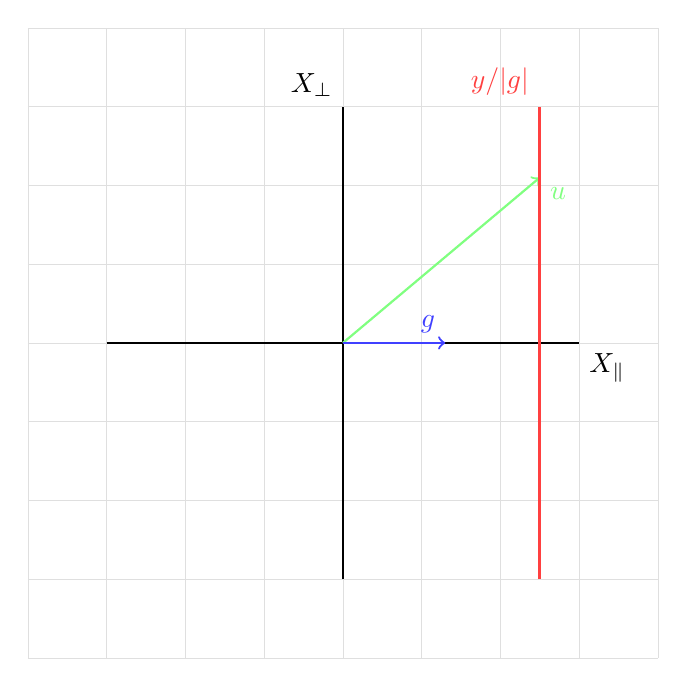
\begin{tikzpicture}
      \draw[step=1cm,gray!25!,very thin] (-4,-4) grid (4,4);
      \draw[thick] (-3,0) -- (3,0) node[anchor=north west] {$X_\parallel$};
      \draw[thick] (0,-3) -- (0,3) node[anchor=south east] {$X_\perp$};
      \draw[green!50,thick,->] (0,0) -- (2.5,2.1) node[anchor=north west] {$u$};
      \draw[blue!75,thick,->] (0,0) -- (1.3, 0) node[anchor=south east] {$g$};
      \draw[red!75,very thick] (2.5,-3) -- (2.5, 3) node[anchor=south east] 
        {$y/|g|$};
  \end{tikzpicture}
  \caption{A linear model in a two-dimensional space is constrained by a single data point $y$. Once the vector $g$ is given, the model is fully specified by the vector $u$, \viz\ $y=g^T u$. All models $u$ along the vertical red line reproduce exactly the data point. In the absence of prior knowledge, every model along that one-dimensional subspace is a legitimate solution of the inverse problem, which is clearly underdetermined.}
  \label{fig:2dexample}
\end{figure}
%
For simplicity we are going to assume that the prior on $\modelvec$ is also a
multi-dimensional Gaussian, centred at $0$ with covariance matrix
$\modelpriorcov$. In this case the posterior distribution can be written as
\begin{equation}
  \label{eq:GaussPostExplicit}
    \pi_{X}^\fwdobsop(\modelvec) 
    \propto \exp \left[
      -\frac{1}{2\gamma^2} \left|\obs - (g^T \modelvec) \right|^2 - \frac12 \left|\modelvec\right|_{\modelpriorcov}^2 
    \right]\, ,
\end{equation}
which is still a Gaussian distribution for $\modelvec$. The mean and covariance
are respectively
\begin{align}
  m &= \frac{(\modelpriorcov g) \obs}{\gamma^2 + (g^T \modelpriorcov g)}\, , \\
  \Sigma &= \modelpriorcov - 
  \frac{(\modelpriorcov g) (\modelpriorcov g)^T}{\gamma^2 + (g^T \modelpriorcov g)}\, .
\end{align}
Because the argument of the exponential is a quadratic form, the mean of the
distribution coincides with the MAP estimator. Hence in this case a fit that
minimises the $\chi^2$ of the data to the theory prediction yields exactly the
mean of the posterior distribution. It is instructive to look at these
quantities in the limit of infinitely precise data, \ie\ in the limit $\gamma\to
0$:
\begin{align}
  m_\star &= 
  \lim_{\gamma\to 0} m
  = \frac{(\modelpriorcov g) \obs}{(g^T \modelpriorcov g)}\, , \\
  \Sigma_\star &= 
  \lim_{\gamma\to 0} \Sigma 
  = \modelpriorcov - 
  \frac{(\modelpriorcov g) (\modelpriorcov g)^T}{(g^T \modelpriorcov g)}\, .
\end{align}
These values satisfy
\begin{align}
  (g^T m_\star) = \obs \, , \\
  (\Sigma_\star g) = 0 \, ,
\end{align}
which shows that the mean of the distribution is such that the data point is
exactly reproduced by the model, and that the uncertainty in the direction
defined by $g$ vanishes. It should be noted that the uncertainty in directions
perpendicular to $g$ does not vanish and is determined by a combination of the
prior and the model, \viz\ $\modelpriorcov$ and $g$ in our example. This is a
particular example of a more general feature: for underdetermined systems the
information from the prior still shapes the probability distribution of the
solution even in the limit of vanishing statistical noise.  

It is interesting to analyse what happens when the prior on the model is
removed. For this purpose we can start from a covariance in model space that is
proportional to the identity matrix, 
\begin{equation}
  \label{eq:DiagCovSigma}
  \modelpriorcov = \sigma \mathbb{1}\, ,
\end{equation}
and take the limit $\sigma \to \infty$. In this limit
\begin{equation}
  \label{eq:LargeSigmaLimit}
  m_\star = y \frac{g}{(g^T g)}\, ,
\end{equation}
while the posterior covariance becomes
\begin{equation}
  \label{eq:ExplcitCov}
  \Sigma_\star= \sigma \left(
    \mathbb{1} - \frac{g g^T}{(g^T g)}
  \right)\, .
\end{equation}
This covariance is the projector on the subspace orthogonal to $g$ multiplied by
$\sigma$. In the simple two-dimensional example depicted in
Fig.~\ref{fig:2dexample}, choosing the direction of $g$ as one of the basis
vector, we obtain
\begin{equation}
  \label{eq:ExplCovTwo}
  \Sigma_\star = 
  \begin{pmatrix}
    0 & \\
    & \sigma
  \end{pmatrix}\, ,
\end{equation}
which shows that the error in the $g$ direction vanishes, while the error in the
orthogonal subspace diverges as we remove the prior. 

\paragraph{Overdetermined system}
We are now going to consider an example of an overdetermined system and discuss
again the case of small observational noise. We consider $\ndata\geq 2$ and
$\nmodel=1$, with a linear forward map such that
\begin{equation}
 \label{eq:OverDetForwMap}
 \obs = g \modelvec  + \obsnoise\, ,
\end{equation} 
where $\obsnoise$ is an $\ndata$-dimensional Gaussian variable with a diagonal
covariance $\gamma^2 \mathbb{1}$, and $\mathbb{1}$ denotes the identity matrix.
For simplicity we are going to assume a Gaussian prior with unit variance for
$\modelvec$, which yields for the posterior distribution:
\begin{equation}
  \label{eq:OverDetPost}
  \pi_{X}^\fwdobsop(\modelvec) 
    \propto 
    \exp\left(
      -\frac{1}{2\gamma^2} \left| \obs - g \modelvec \right|^2
      -\frac12 \modelvec^2
    \right)\, .
\end{equation} 
The posterior is Gaussian and we can easily compute its mean and variance: 
\begin{align}
  m &= \frac{(g^T \obs)}{\gamma^2 + |g|^2} \, , \\
  \sigma^2 &=
    \frac{\gamma^2}{\gamma^2 + |g|^2}\, .
\end{align}
In this case, in the limit of vanishing observational noise, we obtain
\begin{align}
  m_\star &= \frac{(g^T \obs)}{|g|^2} \, ,\\
  \sigma_\star^2 &= 0\, .
\end{align}
The mean is given by the weighted average of the datapoints, which is also the
solution of the $\chi^2$ minimization
\begin{equation}
  m_\star = \arg\min_{\modelvec\in\real} \left|\obs - g \modelvec\right|^2\, .
\end{equation}
Note that in this case the variance $\sigma_\star$ vanishes independently of the
prior. In the limit of small noise, the distribution tends to a Dirac delta
around the value of the MAP estimator.  

\subsection{Linear Problems}
\label{sec:LinProbs}

Linear problems in finite-dimensional spaces are characterized by a simple
forward law, 
\begin{equation}
  \label{eq:MatrixG}
  \obs = \linmap \modelvec\, ,
\end{equation}
where $\linmap$ is a matrix. In this framework one can readily  derive
analytical solutions that are useful to understand the main features of the
Bayesian approach. Assuming that the priors are Gaussian again, the cost
function $S(\modelvec)$ is a quadratic function of $\modelvec$,
\begin{align}
  \label{eq:CostLinGauss}
  S(\modelvec) &= 
  \left(\linmap \modelvec - \obspriorcent \right)^T \obspriorcov^{-1} 
  \left(\linmap \modelvec - \obspriorcent \right) + 
  \left( \modelvec - \modelpriorcent \right)^T \modelpriorcov^{-1} \left(\modelvec - \modelpriorcent \right) \\
  &= 
  \left(\modelvec - \modelpostcent\right) \modelpostcov^{-1}
  \left(\modelvec - \modelpostcent\right) + \mathrm{const}\, ,
\end{align} 
where
\begin{align}
  \label{eq:PostParamsCov}
  \modelpostcov^{-1} &= 
  \left(
    \linmap^T \obspriorcov^{-1} \linmap + \modelpriorcov^{-1}
  \right)\, , \\
  \label{eq:PostParamsMean}
  \modelpostcent &=
  \modelpostcov  \left(
    \linmap^T \obspriorcov^{-1} \obspriorcent + \modelpriorcov^{-1} \modelpriorcent
  \right)\, .
\end{align}
The case where we have no prior information on the model is recovered by taking
the limit $\modelpriorcov^{-1} \to 0$, which yields
\begin{align}
  \label{eq:NoPriorLinModel}
  \modelpostcov^{-1} &= 
  \left(
    \linmap^T \obspriorcov^{-1} \linmap
  \right)\, , \\
  \modelpostcent &=
  \modelpostcov  \left(
    \linmap^T \obspriorcov^{-1} \obspriorcent 
  \right)\, . \label{eq:NoPriorLinModelCov}
\end{align}
The action of $\obspriorcov^{-1}$ on the vector of observed data $\obspriorcent$
is best visualised using a spectral decomposition
\begin{equation}
  \label{eq:CDSpecDec}
  \obspriorcov^{-1} = \sum_n \frac{1}{\sigma_n^2} P_n\, ,
\end{equation}
where $P_n$ denotes the projector on the $n$-th eigenvector of $\obspriorcov$,
and $\sigma_n^2$ is the corresponding eigenvalue. The action of
$\obspriorcov^{-1}$ is to perform a weighted average of the components of
$\obspriorcent$ in the directions of the eigenvectors of $\obspriorcov$.

An explicit expression for the posterior distribution of data can be obtained
from the joint distribution by marginalising over the model input $\modelvec$:
\begin{align}
  \label{eq:PosteriorDataSpace}
  \pi_{Y}^\fwdobsop(\obs|\obspriorcent,\obspriorcov,\modelpriorcent,\modelpriorcov)
  &= \int du\, 
  \pi^\fwdobsop(\obs,\modelvec|\obspriorcent,\obspriorcov,\modelpriorcent,\modelpriorcov) \\
  &\propto \exp\left(
    -\frac12 \left(\obs - \obspostcent\right)^T \obspostcov^{-1}
    \left(\obs - \obspostcent\right)
  \right)\, ,
\end{align}
where
\begin{align}
  \label{eq:PosteriorDataParamsMean}
  \obspostcent &= \linmap \modelpostcent\, , \\
  \label{eq:PosteriorDataParamsCov}
  \obspostcov &= \linmap \modelpostcov \linmap^T\, .
\end{align}
Note that this is the naive error propagation from the covariance of the model,
$\modelpostcov$, to the space of data. 

\paragraph{Posterior distribution of unseen data}

In real-life cases we are also interested in the posterior distribution of a set
of data that have not been included in the fit. Because different datasets are
described by the same theory, the knowledge of one dataset will inform our
knowledge of the underlying theory -- \ie\ we will determine a posterior
distribution for the model. That new knowledge about the model will then
propagate to any other -- unseen -- set of data, even if the experiments are
completely unrelated. In the Bayesian framework that we have developed, this
situation can be modeled by having two independent sets of data $y$ and $y'$,
for which we have a prior distribution 
\begin{align}
  \label{eq:JointIndepDataPrior}
  \pi_{Y}^0&\left(y,y'|y_0,C_{Y},y'_0,C'_{Y}\right) 
   = \pi_{Y}^0\left(y'|y'_0,C'_{Y}\right) \pi_{Y}^0\left(y|y_0,C_{Y}\right) \\
  & \propto 
  \exp\left[-\frac12 \left(y'-y'_0\right)^T (C'_{Y})^{-1} 
  \left(y'-y'_0\right)\right]\, 
  \exp\left[-\frac12 \left(y-y_0\right)^T (C_{Y})^{-1} 
  \left(y-y_0\right)\right]\, .
\end{align}
Note that the prior distribution is factorised as the product of individual
distributions for $y$ and $y'$ since the datasets are assumed to be independent.
Following the derivation above, we can write the joint distribution for the data
and the model 
\begin{equation}
  \label{eq:JointModelData}
  \pi^\fwdobsop(y,y',u) 
  \propto 
  \pi_{Y}^0(y,y'|y_0,C_{Y},y'_0,C'_{Y}) 
  \pi_{X}^0(u) 
  \delta\left(y - \mathcal{G}u\right)
  \delta\left(y'- \mathcal{G}'u\right)\, .
\end{equation}
Because both sets of data are derived from the same model $u$, the joint
distribution above introduces a correlation between the data sets. The same
model $u$ appears in both delta functions in the equation above. We can now
marginalise with respect to the dataset $y$, 
\begin{equation}
  \label{eq:MarginaliseDatasetY}
  \begin{split}
    \pi(y',u) 
    \propto &
    \exp\left[-\frac12 \left(y'-y'_0\right)^T (C'_{Y})^{-1} 
    \left(y'-y'_0\right)\right]\, 
    \exp\left[-\frac12 \left(u-\tilde{u}\right)^T (\tilde{C}_{X})^{-1} 
    \left(u-\tilde{u}\right)\right] \\
    & \quad \times \delta\left(y'- \mathcal{G}'u\right)\, .
  \end{split}
\end{equation}
where $\tilde{C}_{X}$ and $\tilde{u}$ are given respectively in
Eqs.~\ref{eq:PostParamsCov} and \ref{eq:PostParamsMean}. By marginalising again,
this time with respect to the model, we derive the posterior distribution of the
unseen data,
\begin{equation}
  \label{eq:MarginaliseModelU}
  \pi^y_{Y}(y') \propto 
  \exp \left[ 
   \frac12 \left(y' - \tilde{y}'\right)^T
   (\tilde{C}'_{Y})^{-1} 
   \left(y' - \tilde{y}'\right)
   \right]\, ,
\end{equation}
where
\begin{align}
  \label{eq:lineone}
  \tilde{C}'_{Y} 
  &= \mathcal{G}' \tilde{C}'_{X} \mathcal{G}'^{T} \\
  \label{eq:linetwo}
  \tilde{y}'
  &= \mathcal{G}' \tilde{u}'\, ,
\end{align}
and we have introduced the variables $\tilde{u}'$ and $\tilde{C}'_{X}$,  
\begin{align}
  \label{eq:ModelPostSequential}
  \tilde{C}_{X}'^{-1} 
  &= \mathcal{G}'^T C_{Y}'^{-1} \mathcal{G}' + \tilde{C}_{X}^{-1} \\
  \label{eq:ModelPostSequentialTwo}
  \tilde{u}' 
  &= \tilde{C}'_{X} \left(
    \mathcal{G}'^T C_{Y}'^{-1} y_0' + \tilde{C}_{X}^{-1} \tilde{u} 
    \right) \, .
\end{align}
The variables $\tilde{C}_{X}$ and $\tilde{u}$ have been defined above. We repeat
their definition here in order to have all the necessary equations collected
together: 
\begin{align}
  \label{eq:linethree}
  \tilde{C}_{X}^{-1}
  &= \mathcal{G}^T C_{Y}^{-1} \mathcal{G} + C_{X}^{-1} \\
  \label{eq:linefour}
  \tilde{u}
  &= \tilde{C}_{X} \left(
    \mathcal{G}^T C_{Y}^{-1} y_0 + C_{X}^{-1} u_0
  \right)\, .
\end{align}
Eqs.~\ref{eq:lineone}, \ref{eq:linetwo}, \ref{eq:ModelPostSequential},
\ref{eq:ModelPostSequentialTwo}, \ref{eq:linethree} and \ref{eq:linefour} yield
the central value and the variance of the posterior distribution of unseen data
as a function of $y_0$, $y_0'$, $C_Y$, $C_Y'$, $u_0$ and $C_X$. 

\paragraph{A comment on non-linear models}

The linear models that we have discussed so far may look over-simplified at
first sight. In practice, it turns out that non-linear models can often be
linearised around the central value of the prior distribution, 
\begin{equation}
  \label{eq:LinU0}
  \fwdobsop(\modelvec) = \fwdobsop(\modelpriorcent) + G \left(\modelvec - \modelpriorcent\right) + \ldots\, ,
\end{equation}
where 
\begin{equation}
  \label{eq:FirstDerU0}
  G^i_\alpha = \left. \frac{\partial \fwdobsop^i}{\partial u_\alpha} \right|_{\modelpriorcent}\, ,
\end{equation}
and we have neglected higher-order terms in the expansion of
$\fwdobsop(\modelvec)$.

If these terms are not negligible, another option is to find the MAP estimator,
and then expand the the forward map around it, which yields equations very
similar to the previous ones, with $\modelpriorcent$ replaced by $u_*$. If the
posterior distribution of $u$ is sufficiently peaked around the
MAP estimator, then the linear approximation can be sufficiently accurate. 


\subsection{The infinite-dimensional case}
\label{sec:infin-dimens-case}

In the finite-dimensional case, where the probability measures are specified by
their densities with respect to the Lebesgue measure,
Eq.~(\ref{eq:BayesThmInversePosterior}) can be rephrased by saying  that $\rho$
is the Radon-Nikodym derivative of the probability measure $\mu^\fwdobsop$ with
respect to $\mu_0$, \viz
\begin{align}
  \label{eq:RadonNikodym}
  \frac{d\mu^\fwdobsop}{d\mu^0} (\modelvec) \propto \rho(\obs-\fwdobsop(\modelvec))\, .
\end{align}
Using the fact that the density $\rho$ is a positive function, we can rewrite 
\begin{align}
  \label{eq:PotentialDef}
  \rho(\obs-\fwdobsop(\modelvec)) = \exp\left(-\Phi(\modelvec;\obs)\right)\, ,
\end{align}
and therefore
\begin{align}
  \label{eq:RadonNikodymTwo}
  \frac{d\mu^\fwdobsop}{d\mu^0} (\modelvec) \propto \exp\left(-\Phi(\modelvec;\obs)\right)\, .
\end{align}
In finite-dimensional spaces, the three equations above are just definitions
that do not add anything to the above discussion in terms of probability
densities. Their interest resides in the fact that the last expression,
Eq.~(\ref{eq:RadonNikodymTwo}), can be properly defined when $\modelspace$ is
infinite-dimensional, allowing a rigorous extension of the Bayesian formulation
of inverse problems to the case of infinite-dimensional spaces. 

Summarising the details of probability measure in infinite-dimensional spaces,
is beyond the scope of this work. Adopting instead a heuristic approach, we can
say that a function $f$ is a random function if $f(x)$ is a random variable for
all values of $x$. Since the values of the function at different values of $x$
can be correlated, a random function is fully characterised by specifying the
joint probability densities
\begin{equation}
  \label{eq:RandomFuncJointProb}
  \pi\left(
    f_1, \ldots, f_n; x_1, \ldots x_n
  \right)\, ,
\end{equation}
where $f_i=f(x_i)$, for all values of $n$, and all values of $x_1, \ldots, x_n$.
This infinite set of finite-dimensional densities allows the definition of a
probability measure. 

For a Gaussian random function, these densities only depend on a mean value
function $m(x)$ and a covariance $C(x,x')$. The probability densities for the
variables $f_i$, for any value of $n$ is 
\begin{equation}
  \label{eq:GaussianFunctC}
  \pi\left(f_1, \ldots, f_n; x_1, \ldots, x_n\right)
  \propto \exp \left[ 
      -\frac12 \sum_{ij} \left(f_i - m_i\right) C^{-1}(x_i,x_j) \left(f_j - m_j\right)
    \right]\, .
\end{equation} 
The covariance $C$ is such that
\begin{equation}
  \label{eq:CovFunctInt}
  C(x,x') = \int df\, df'\, \left(f - m(x)\right) \left(f'-m(x')\right)
    \pi\left(f,f';x,x'\right)\,,
\end{equation}
which shows that the two-point probability density determines all the other
distributions. 

\paragraph{Functional linear problems} This formalism allows us to formulate a
Bayesian solution of the inverse problem 
\begin{equation}
  \label{eq:BayesLinearInverse}
  y^i = \int dx\, G^i(x) u(x)\, ,
\end{equation}
where $y^i$ is a discrete set of observables and $u(x)$ is a random function,
with a Gaussian prior with mean $u_0(x)$ and covariance $C_{X}(x,x')$. The
vector of observed values is denoted $y_0$, and we assume that the prior
distribution of $y$ is a Gaussian centred at $y_0$ with covariance $C_{Y}$.

Similarly to the finite-dimensional case, the Bayesian solution yields a
Gaussian random function for the posterior distribution of the solution $u(x)$.
In order to characterise the posterior Gaussian distribution we need explicit
expressions for its mean and its covariance. Introducing the matrix
\begin{equation}
  \label{eq:Smatrix}
  S^{ij} =
  \int dx dx'\, G^i(x) C_{X}(x,x') G^j(x') + C_{Y}^{ij}\, ,
\end{equation}
and its inverse $T^{ij}=\left(S^{-1}\right)^{ij}$, the posterior Gaussian field
is centred at
\begin{align}
  \label{eq:PostMeanFunc}
  \tilde{u}(x) = u_0(x) + 
  \int dx'\, C_{X}(x,x') G^i(x') T^{ij} \left(
    y_0^j - \int dx''\, G^j(x'') u_0(x'') 
  \right)\, ,
\end{align}
which is the expected generalization of the finite-dimensional example discussed
above. Interestingly, this can be rewritten as
\begin{equation}
  \label{eq:TowardsBackus}
  \tilde{u}(x) = u_0(x) + 
  \int dx'\, C_{X}(x,x') \psi(x')\, ,
\end{equation}
where 
\begin{eqnarray}
  \label{eq:PsiDef}
  \psi(x) = G^i(x) \delta y^i\, ,
\end{eqnarray}
and the weighted residuals are given by
\begin{equation}
  \label{eq:DeltaYDef}
  \delta y^i = T^{ij} \left(
  y_0^j - \int dx'\, G^j(x') u_0(x')
  \right)\, .
\end{equation}
Defining 
\begin{equation}
  \label{eq:CapitalPsi}
  \Psi^i(x) = \int dx'\, C_{X}(x,x') G^i(x')\, ,
\end{equation}
the posterior covariance can be written as
\begin{equation}
  \label{eq:PostCovFunc}
  \tilde{C}_{X}(x,x') = 
  C_{X}(x,x') - \Psi^i(x) T^{ij} \Psi^j(x')\, .
\end{equation}

It is instructive to compare the Bayesian result summarised above with the
method proposed by Backus and Gilbert~\cite{BackusGilbert1968} to solve the same
inverse problem. Assuming that there exists an unknown 'true' model $\utrue$,
such that the observed data are
\begin{equation}
  \label{eq:BackStart}
  y_0^i = \int dx\, G^i(x) \utrue(x)\, ,
\end{equation}
we look for an estimate $\uest$ of the true solution in the form
\begin{equation}
  \label{eq:BackAnsatz}
  \uest(x) = Q^i(x) y^i_0\, ,
\end{equation}
so that the problem is now recast as finding the functions $Q^i(x)$.
Using Eq.~\ref{eq:BackStart} we obtain
\begin{equation}
  \label{eq:BackFilter}
  \uest(x) = \int dx' R(x,x') \utrue(x')\, , 
\end{equation}
which states that with a finite amount of data we can only resolve a filtered
version of the true solution. The kernel $R$ is given by
\begin{equation}
  \label{eq:BackKernel}
  R(x,x') = Q^i(x) G^i(x')\, .
\end{equation}
The coefficient functions $Q^i(x)$ can be chosen so that the kernel is as close as possible
to a delta function,
\begin{equation}
  \label{eq:BackDelta}
  R(x,x') \simeq \delta(x,x') ~~ \Longrightarrow ~~
  \uest \simeq \utrue\, .
\end{equation}
Approximating the delta function can be achieved by minimising 
\begin{equation}
  \label{eq:BackDeltaness}
  \int dx'\, \left(
    R(x,x') - \delta(x-x')
  \right)^2\, ,
\end{equation}
which yields
\begin{equation}
  \label{eq:BackSolution}
  Q^i(x) = \left(S^{-1}\right)^{ij} G^j(x)\, ,
\end{equation}
where 
\begin{equation}
  \label{eq:BackSMatrix}
  S^{ij} = \int dx\, G^i(x) G^j(x)\, .
\end{equation}
The interesting observation is that the central value of the Bayesian solution
presented above reduces to the Backus-Gilbert $\uest$ in the case where $u_0$ 
is just white noise and therefore
\begin{equation}
  \label{eq:BackComparison}
  C_{X}(x,x') = \delta(x-x')\, .
\end{equation}
The connections between the Bayesian treatment and the Backus-Gilbert solution
and its regulated variations, deserves further investigations, which we defer to
future studies. Note that the Bayesian solution allows a variety of priors to be
explicitly declared and compared to the Backus-Gilbert solution. 